\section{Couchsurfing \cite{couchsurfing}}
\label{analyza:couchsurfing}

Ubytování bývá drahé a proto existují lidé, kteří na pár nocí vypůjčují svůj gauč a tím pomohou někomu poznat jejich město a zemi. Pro cestující z toho plyne ještě jeden pozitivní dopad -- skvělé informace, které by se nikde jinde nedozvěděli, a to přímo od lokálního člověka.\\

\subsection{Hlavní stránka}
\begin{figure}[h]
    \centering
    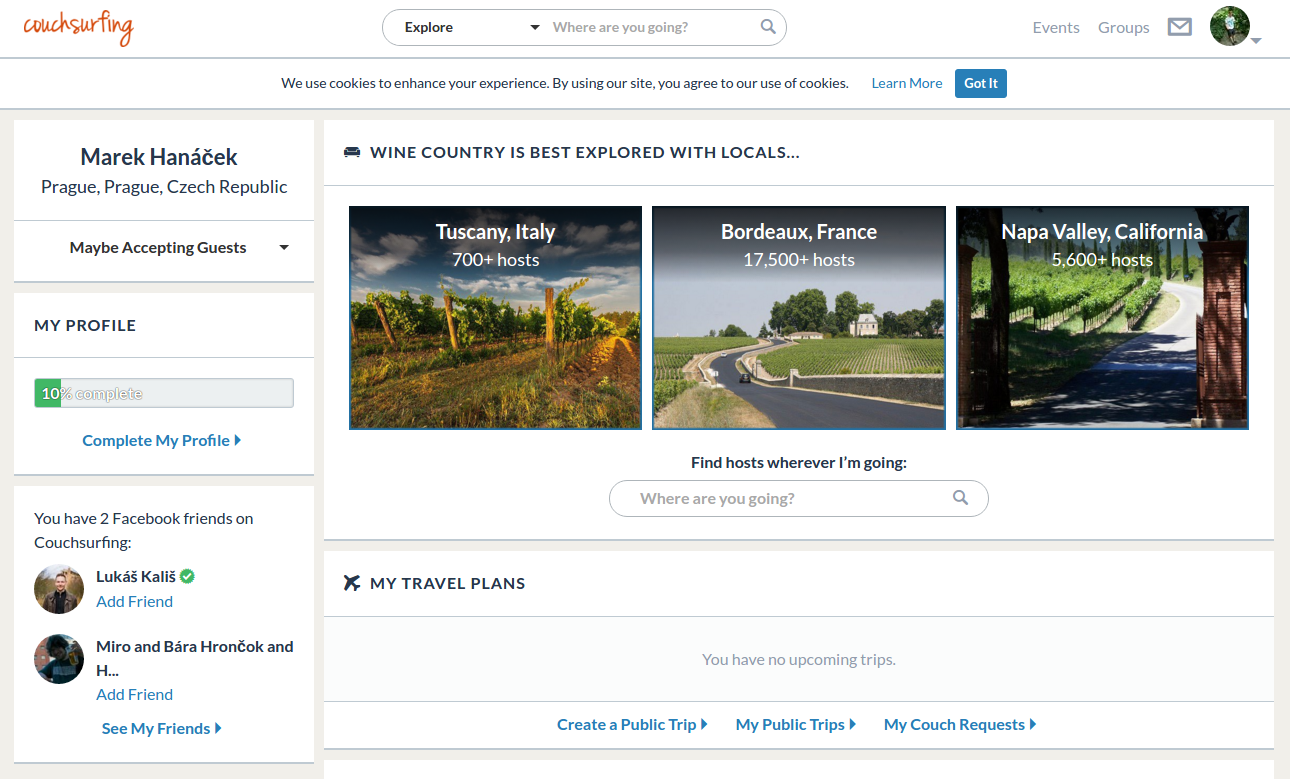
\includegraphics[width=1.0\textwidth]{media/couchsurfing/homepage.png}
    \caption{Hlavní stránka webu couchsurfing.cz}
    \label{fig:couchsurfing:homepage}
\end{figure}
\subsubsection*{Pozitiva}
\begin{itemize}
    \item[+] \textbf{Přehlednost} -- Všechno důležité na jednom místě a přehledně oddělené.
    \item[+] \textbf{Vyhledávací okno} -- Rychlé vyhledávací okno v horní části stránky.
\end{itemize}
\subsubsection*{Negativa}
\begin{itemize}
    \item[-] \textbf{Stránka je dlouhá} -- Pro zobrazení veškerého obsahu je potřeba dlouho točit kolečkem myši.
\end{itemize}


%%%%%%%%%%%%%%%%%%%%%%%%%%%%%%%%%%%%%%%%%%%%%%%%%%%%%%%%%%%%%%%%%%%%%%%%%%%%%%%%%%%%%%%%%%%%%%%%%%%%%%%%%%%%%%%%%%%%%%%%

\newpage
\subsection{Vyhledávání ubytovaní}
\begin{figure}[h]
    \centering
    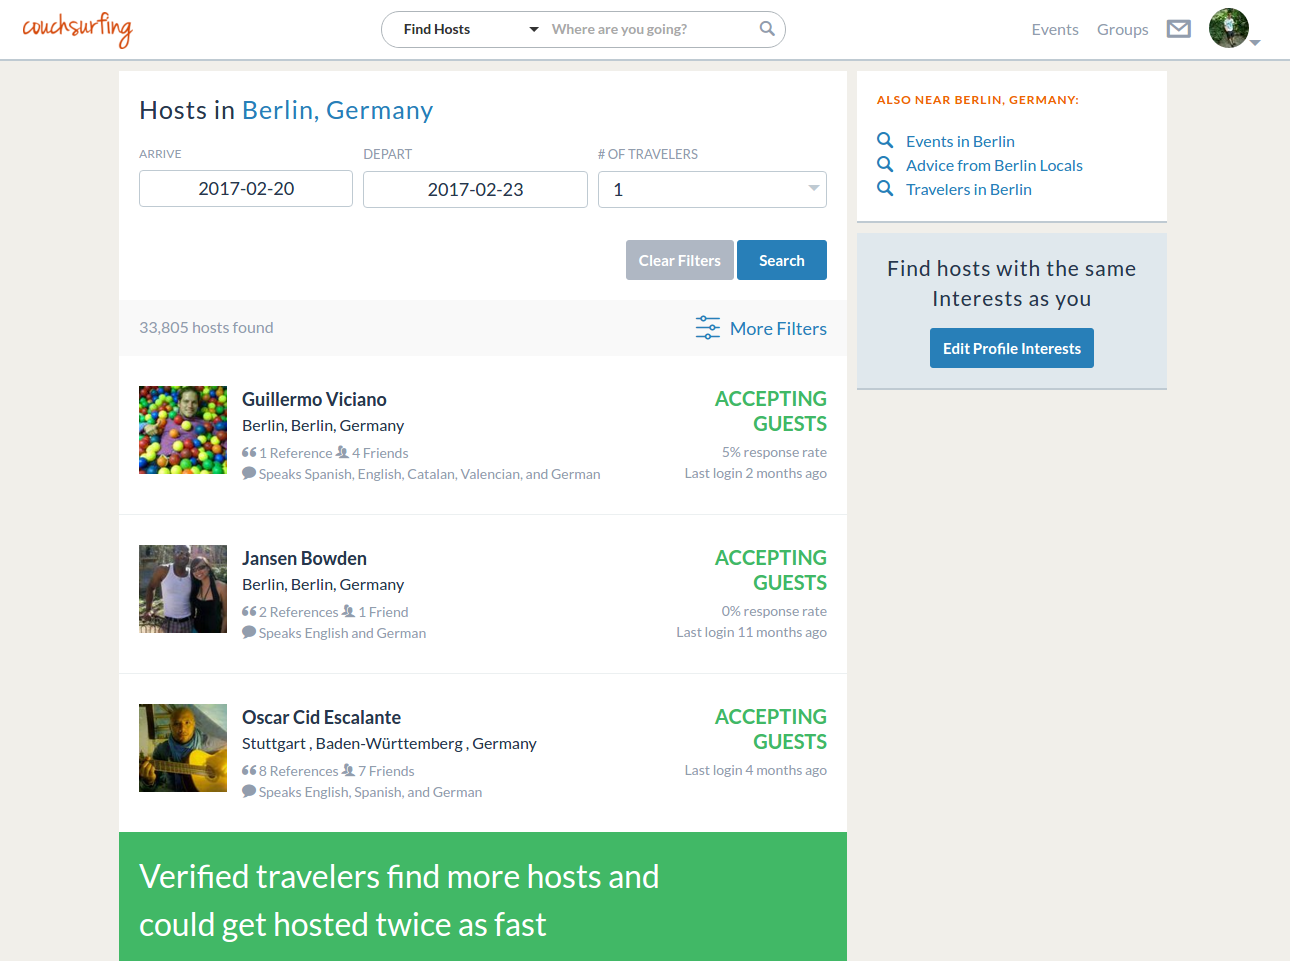
\includegraphics[width=1.0\textwidth]{media/couchsurfing/search.png}
    \caption{Vyhledávání ubytování na webu couchsurfing.cz}
    \label{fig:couchsurfing:search}
\end{figure}
\subsubsection*{Pozitiva}
\begin{itemize}
    \item[+] \textbf{Jednoduchost}
    \item[+] \textbf{Filtry} -- Všechno důležité s možností rozšířeného filtru.
    \item[+] \textbf{Status} -- Ověření uživatelé jsou jasně viditelní.
\end{itemize}
\subsubsection*{Negativa}
\begin{itemize}
    \item[-] \textbf{Nevidím}
\end{itemize}


%%%%%%%%%%%%%%%%%%%%%%%%%%%%%%%%%%%%%%%%%%%%%%%%%%%%%%%%%%%%%%%%%%%%%%%%%%%%%%%%%%%%%%%%%%%%%%%%%%%%%%%%%%%%%%%%%%%%%%%%

\newpage
\subsection{Profil}
\begin{figure}[h]
    \centering
    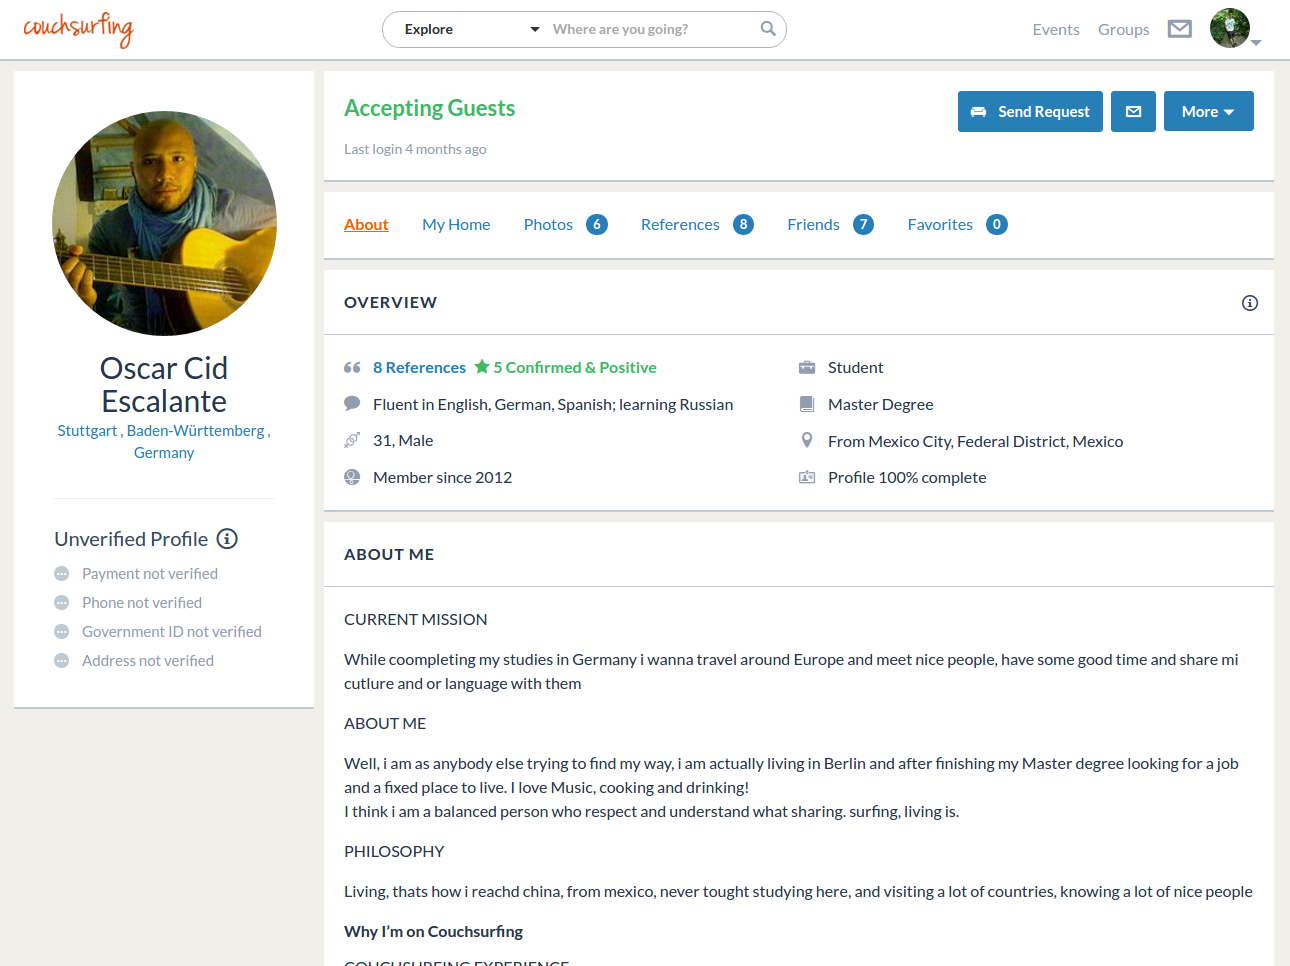
\includegraphics[width=1.0\textwidth]{media/couchsurfing/profile.png}
    \caption{Profil uživatele na webu couchsurfing.cz}
    \label{fig:couchsurfing:profile}
\end{figure}
\subsubsection*{Pozitiva}
\begin{itemize}
    \item[+] \textbf{Informativnost} -- Všechno kompaktně na jednom místě a přehledně.
    \item[+] \textbf{About me} -- To zda mi daný člověk bude vyhovovat častokrát zjistíme už z toho jak dokáže popsat sám sebe. Určitě vítaná funkcionalita.
\end{itemize}
\subsubsection*{Negativa}
\begin{itemize}
    \item[-] \textbf{Nevidím}
\end{itemize}


%%%%%%%%%%%%%%%%%%%%%%%%%%%%%%%%%%%%%%%%%%%%%%%%%%%%%%%%%%%%%%%%%%%%%%%%%%%%%%%%%%%%%%%%%%%%%%%%%%%%%%%%%%%%%%%%%%%%%%%%

\newpage
\subsection{Shrnutí}
Celkově se mi webová aplikace Couchsurfing jeví velmi dobře řešená.\\

Důležitým mottem, s kterým buduji webovou aplikaci, je být \textbf{přehledný}. Každá podstránka by měla obsahovat všechno co je potřeba a nic víc. Zajímavou myšlenkou se mi jeví existence \textbf{verifikovaných uživatelů}, která by v této práci vytvořila důvěru a určitou záruku korektního jednání při výměně peněz. Nevýhodu vidím ve velmi dlouhém provedení úvodní stránky, čehož se budu snažit vyvarovat a tím pádem ulehčit uživateli orientaci na stránce.